\chapter{The Analytical N-BPM method}
\label{ch_anbpm}

\begin{chapterinfo}
One of the most important figures of merit of optics correction is the deviation of the real $\beta$~function
from the model values,
the $\beta$~\emph{beating}. A deviation from the ideal values has a negative effect on machine performance.
Too high $\beta$~beating can even put machine components in danger and a threshold for operation with
physics filling scheme has to be imposed for machine protection reasons.

Furthermore, large $\beta$~beating deteriorates other linear and especially non-linear optics measurements
and correction methods. Therefore a good control of the $\beta$~beating can be essential for higher-order
correction steps.

This chapter summarises classical $\beta$~beating methods from turn-by-turn data in section~\ref{sec_classical_beta_meas}
and describes in detail a new algorithm, the \emph{analytical N-BPM method},
which improves speed and performance by calculating analytically the error propagation
in sections~\ref{sec_corrected_beta_from_phase} through \ref{sec_corr_matr}.
Accuracy and precision of the new method are assessed using simulations of current LHC optics and design
optics for the High-Luminosity upgrade of the LHC in sections~\ref{sec_bad_combs} and \ref{sec_hllhc_nbpm}.

With the exception of the first two sections, which set the context of the present study and introduce the
mathematical tools, this chapter represents original work.

The content of this chapter has been published in~\cite{Wegscheider2017}.

\end{chapterinfo}

\section{\texorpdfstring{$\beta$}{beta}~function measurement from turn-by-turn data}
\label{sec_classical_beta_meas}

\subsection{Three BPM method}

The classical method to measure the $\beta$~function in hadron machines is the \emph{Three BPM Method}
introduced in section~\ref{sec_beta_meas}.



With this method one can use the phase advance between three BPMs $i,j,k$ to calculate the $\beta$~function
of the probed BPM $i$. It is a model dependent approach, the greater the difference between the model
and the real accelerator the less accurate will be the result. A good knowledge of the actual accelerator
is crucial for this approach to work.

\equationref{eq_3bpm_method} has been developed for LEP and it has been used for optics measurements in LEP
and LHC during run I.
But it has two shortcomings: it assumes that the actual $\beta$~beating is very low and it
diverges for phase advances close to $n\pi$, $n \in \mathbb{N}$. The latter makes measurements at
exact $n\pi$ phase advances impossible and strongly enhances phase measurement errors near $n\pi$.
Unfortunately, especially in the IR phase advances are very small and precise $\beta$~function measurements
are not feasible.

%\begin{wrapfigure}{O}[\figborderhang]{6cm}
\begin{figure}
    \centering
    \includestandalone{figThreeBPM} 
    \caption{A sketch of the three BPM method. The probed BPM is shown in blue. For LHC arcs the
    combination with the probed BPM in the center is the most stable against phase measurement errors.}
    \label{fig_threebpm}
\end{figure}
%
\figureref{fig_threebpm} displays a sketch of the Three BPM Method. The probed BPM is shown in blue,
BPMs $j$ and $k$ are shown in red.
Classically the arithmetic mean of all three adjacent cases -- as shown in the figure -- were used.


In LHC arcs where the phase advance between adjacent BPMs is around
$\SI{45}{\degree}$ the combination with the probed BPM in the center yields almost optimal results
since the perturbation from phase measurement errors is small for the occurring phase advances.
The two other cases shown in \figref{fig_threebpm} on the other hand include the 
phase advance $\phi_{13} = \SI{90}{\degree}$ which is less optimal.

In LHC interaction regions the phase advance between consecutive BPMs does not follow the same constraints
as in the arc and values different from $\SI{45}{\degree}$ may appear. In the final focus quadrupoles
the $\beta$~function peaks are very high to deliver a strong focusing of the beams in the interaction
point\footnote{cf. Fig.~\ref{fig_beta}}. This yields a very small phase advance in this area, rendering a $\beta$ measurement from phase
impossible. At the same time a high precision of $\beta$~beating is necessary to control $\betastar$ and
to optimise the aperture.

\subsection{Original N-BPM method}

To avoid cases with unsuitable phase advances or to get the optimal phase advances, BPMs can be
skipped. For an LHC arc a combination as shown in \figref{fig_skip_one_BPM} can be used for the non-center
cases of the Three BPM method in order to have the least uncertainties in all three combinations.

A second tool that can be applied to reduce uncertainty is averaging over more combinations which
improves statistics and reduces statistical uncertainties.
Unfortunately, systematic errors increase
as more and more BPMs are skipped because of the presence of other elements with their imperfections in between the
BPMs.
In order to further improve the precision the information about statistical and systematic
uncertainties can be used to calculate a weighted mean:
%
\begin{align}
    \beta(s_i) &= \sum\limits_{l} \beta_l(s_i) g_l
    \label{eq_beta_wmean}\\
    \beta_l(s_i) &=
        \frac{
            \cot\phi_{ij_l} - \cot\phi_{ik_l}
        }{
            \cot\phi_{ij_l}\m - \cot\phi_{ik_l}\m
        } \beta(s_i)\m
    \komma
    \label{eq_beta_l}
\end{align}
%
with the weights $g_l$ satisfying
%
\begin{equation}
    \sum\limits_l g_l = 1
    \komma
\end{equation}
%
and $j_l,\,k_l$ pairs of BPMs around the probed BPM.


%\begin{wrapfigure}{O}[\figborderhang]{7cm}
\begin{figure}
    \centering
    \includestandalone{figSkipOneBpm}
    \caption{In the LHC arcs skipping one BPM for the non-center cases of the Three BPM Method
    is of advantage since the phase advance $\phi_{14}$
    is more suitable regarding error propagation.}
    \label{fig_skip_one_BPM}
\end{figure}
%
Furthermore the $\beta$~function values calculated from different combinations are not statistically
independent and correlation has to be taken into account when calculating the weights.
The N-BPM method \cite{LangnerNBPM, Langner2017} was developed to implement this feature.
It was successfully used in the LHC during run II and for the re-analysis of run I data
as well as in the storage rings of ALBA and ESRF.

The name originates in the fact that the BPMs $i$, $j_l$ and $k_l$ are taken in a range of $N$ BPMs.
This generates $n = (N-2)(N-1)/2$ combinations.

% --------------------------------------------------------------------------------------------------
% Generalised least squares
% --------------------------------------------------------------------------------------------------
\section{Generalised least squares}

To get the correct estimate for the weights $g_l$ the study of some statistics is in order.
The weights can be determined using a least-squares optimisation. The weighted mean \eqref{eq_beta_wmean}
can be rewritten in vector notation:
%
\begin{align}
    \vec{\hat{\beta}} &= \mat{B}\vec{\gamma}
    \label{eq_beta_wmean_vec}\\
    \vec{\hat{\beta}} &= 
    \begin{pmatrix}
        \hat{\beta}\\
        \vdots\\
        \hat{\beta}
    \end{pmatrix},\quad
    \vec{\gamma} =
    \begin{pmatrix}
        g_1\\
        \vdots\\
        g_n
    \end{pmatrix},\quad
    \mat{B} =
    \begin{pmatrix}
        \vec{\beta}^T\\
        \vdots\\
        \vec{\beta}^T
    \end{pmatrix}
    \komma
\end{align}
%
where each line of the equation system is just the same.
The difference between measurement $l$ and the mean value $\hat{\beta}$ is denoted by $\epsilon_l$:
%
\begin{equation}
    \vec{\epsilon} = \vec{\hat{\beta}} - \vec{\beta}
    \fstop
\end{equation}
%
The least square minimisation seeks a set of weights $g_i$ for which the squared errors are minimal. Since the different $\beta_l$
are correlated and have a covariance matrix $\mat{Cov}[\vec{\beta}] \neq \mat{diag}(\sigma_1^2, \ldots, \sigma_n^2)$
the theory of generalised least-squares estimation~\cite{kariya2004generalized} has to be applied.

The \emph{covariance matrix} of a set of random variables $\Omega_i$ is defined as
%
\begin{align}
    \mat{Cov}[\vec{\Omega}] &= \mat{E}[(\vec{\Omega} - E[\vec{\Omega}])(\vec{\Omega} - E[\vec{\Omega}])^T]
    \notag \\
    &= \mat{E}[\vec{\Omega}\vec{\Omega}^T] - E[\vec{\Omega}]E[\vec{\Omega}]^T
    \komma
    \label{eq_def_cov}
\end{align}
%
where $E[\vec{\Omega}]$ is the \emph{expected value} of the random variables $\vec{\Omega}$. And the
notation is chosen such that the expected value of a vector is a vector
of expected values of each component and similar for matrices.

\equationref{eq_def_cov} can be expressed element-wise:
%
\begin{equation}
    \left(Cov[\vec{\Omega}]\right)_{ij} = E[\Omega_i\Omega_j] - E[\Omega_i]E[\Omega_j]
    \label{eq_cov_form}
    \fstop
\end{equation}
%
\subsection{Error Propagation}

Consider a set of unperturbed phase measurements $ \{\phi_1, \ldots, \phi_n\} $ and non-observable  parameters $  \{ K_{1,1} , \ldots , K_{1,m}, s_1, \ldots, s_{\nu}, x_1, \ldots x_{\mu} \} $ with corresponding errors $ \Delta \phi_\alpha,\, \Delta K_{1,\beta}, \,\Delta s_\gamma,\, \Delta x_\kappa  $.
Collecting all parameters into a vector
%
\begin{equation}
\vec{\Omega}_0 =
\begin{pmatrix}
\vec{\phi}\\
\vec{K}\\
\vec{s}\\
\vec{x}
\end{pmatrix},\quad
\vec{\Delta \Omega} = 
\begin{pmatrix}
\vec{\Delta\phi}\\
\vec{\Delta K}\\
\vec{\Delta s}\\
\vec{\Delta x}
\end{pmatrix}
\fstop
\end{equation}
%
Using a Taylor expansion the errors in these parameters can be propagated
%
\begin{equation}
\beta_l (\vec{\Omega}) = \beta_l(\vec{\Omega}_0) + \partial^i\beta_l(\vec{\Omega}_0)\Delta\Omega_i +  \partial^i\partial^j\beta_l(\vec{\Omega}_0)\Delta\Omega_i\Delta\Omega_j + O(\Delta\Omega^3)\;,
\label{eq:err_prop}
\end{equation}
%
where the Einstein summation convention is used and the derivatives are w.r.t. $ \Omega_i $: $ \partial^i\beta_l \equiv \frac{\partial \beta_l}{\partial \Omega_i} $.
The argument $ (\vec{\Omega}_0) $ is omitted in the following for the $ \beta $ function and its derivatives at the unperturbed position $ \vec{\Omega}_0 $. For the calculation of the covariance matrix,
\eqref{eq:err_prop} is truncated to second order and for convenience and readability,
the two summands of \eqref{eq_cov_form} are derived separately.
%
\begin{equation}
E[\beta_l(\vec{\Omega})] \approx E\left[   
\beta_l + \partial^i\beta_l\Delta\Omega_i +  \partial^i\partial^j\beta_l\Delta\Omega_i\Delta\Omega_j 
\right] =
\beta_l + \partial^i\beta_l E[\Delta\Omega_i] +  \partial^i\partial^j\beta_l E\left[\Delta\Omega_i\Delta\Omega_j \right]\;.
\end{equation}
%
 It is assumed that there are no systematic errors in the measurement instruments and so $ {E}[{\Delta\Omega_i}] =0$ and the middle term vanishes.
One can conclude
%
\begin{equation}
E[\beta_l(\vec{\Omega})]E[\beta_m(\vec{\Omega})] \approx \beta_l\beta_m +
 \left(\beta_l\partial^i\partial^j\beta_m +
 \beta_m\partial^i\partial^j\beta_l\right) E\left[\Delta\Omega_i\Delta\Omega_j \right]\;,
 \label{eq:Eb_Eb}
\end{equation}
%
 where terms proportional to the square of the variance go into the reminder $ O(\Delta\Omega^3) $.

To calculate the term $ {E}[{\beta_l}{\beta_m}] $ more steps are needed:
%
\begin{align}
E\left[\beta_l(\vec{\Omega})\beta_m(\vec{\Omega})\right]& = 
E\left[
	(
		\beta_l + \partial^i\beta_l\Delta\Omega_i + \partial^i\partial^j\beta_l\Delta\Omega_i\Delta\Omega_j
	)
	(
		\beta_m + \partial^i\beta_m\Delta\Omega_i + \partial^i\partial^j\beta_m\Delta\Omega_i\Delta\Omega_j
	)
\right] \notag \\
&\approx E\left[
	\beta_l\beta_m + 
	\left(\beta_l\partial^i\beta_m + \beta_m\partial^i\beta_l\right)\Delta\Omega_i +
	\partial^i\beta_l\partial^j\beta_m\Delta\Omega_i\Delta\Omega_j +\right. \notag\\ &\left.\quad\quad\quad
	\left(\beta_l\partial^i\partial^j\beta_m +\beta_m\partial^i\partial^j\beta_l\right)\Delta\Omega_i\Delta\Omega_j
\right] \notag\\
&= 	
	\beta_l\beta_m + 
	\partial^i\beta_l\partial^j\beta_mE[\Delta\Omega_i\Delta\Omega_j]+
	\left(\beta_l\partial^i\partial^j\beta_m +
	\beta_m\partial^i\partial^j\beta_l\right) E\left[\Delta\Omega_i\Delta\Omega_j \right]\;.
	\label{eq:Ebb}
\end{align}
%
Finally, subtracting \eqref{eq:Eb_Eb} from \eqref{eq:Ebb}, yields
%
\begin{equation}
(\text{Cov}[\vec{\beta}])_{lm} = \partial^i\beta_l\partial^j\beta_mE[\Delta\Omega_i\Delta\Omega_j] = \partial^i\beta_l\partial^j\beta_m \text{Cov}[\vec{\Delta\Omega}]_{ij}\;.
\label{eq:covbb}
\end{equation}
%
In the last step again the assumption $ E(\Delta\Omega_i)=0 $ is made, implying
%
\begin{equation}\label{eq_cov}
\text{Cov}[\vec{\Delta\Omega}]_{ij} =  E\left[\Delta\Omega_i \right] E[\Delta\Omega_j ] -  E\left[\Delta\Omega_i\Delta\Omega_j \right] =  E\left[\Delta\Omega_i\Delta\Omega_j \right]\;.
\end{equation}
%
In matrix notation \eqref{eq:covbb} reads
%
\begin{equation}
\mat{Cov}\left[\vec{\beta}\right] = \mat{T}\; \mat{Cov}\left[\vec{\Delta\Omega}\right] \;\mat{T}^T,
\end{equation}
%
 where 
%
\begin{equation}
T_{ij} = \frac{\partial \beta_i}{\partial \Omega_j}\;.
\end{equation}
%
If the parameters $ \vec{\Omega} $ are uncorrelated, the covariance matrix of $\vec{ \Delta\Omega} $ simplifies to
%
\begin{align}
\left(\text{Cov}\left[\vec{\Delta\Omega}\right] \right)_{ij}&= 0 \quad  \text{ if } i\neq j \;,\\
 \left(\text{Cov}\left[\vec{\Delta\Omega}\right] \right)_{ii}&= \sigma_i^2\;,
\end{align}
%
%
\begin{equation}
\Rightarrow E\left[\Delta\Omega_i\Delta\Omega_j\right] = E\left[\Delta\Omega_i\right]E\left[\Delta\Omega_j\right]\quad \text{ if } i \neq j\;,
\end{equation}
%
and \eqref{eq:covbb} reads
%
\begin{equation}
(\text{Cov}[\vec{\beta}])_{lm} = \partial^i\beta_l\partial^i\beta_mE[\Delta\Omega_i^2] = \partial^i\beta_l\partial^i\beta_m \sigma_i^2\;,
\end{equation}
%
with the variance being defined by
%
\begin{equation}
\sigma_i^2 = E\left[\Delta\Omega_i^2\right]
\fstop
\end{equation}
%
\subsection{The generalised least-squares estimator}

After computing the covariance matrix of $ \beta $, the generalised least-squares estimator can be calculated
by solving the translated system
%
\begin{equation}
\mat{X}^{-1} \vec{\beta} = \mat{X}^{-1}\mat{B}\vec{\gamma} + \mat{X}^{-1}\vec{\epsilon}
\end{equation}
%
where the translation $ \mat{X} $ is such that $ \mat{X}^T\mat{X} = \mat{V} = \mat{Cov}[\vec{\beta}] $. The least-squares estimation searches for a minimum of 
%
\begin{equation}
\left\|\mat{X}^{-1}\left(\vec{\beta} - \mat{B}\vec{\gamma}\right)\right\|^2 = \left(\vec{\beta} - \mat{B}\vec{\gamma}\right)^T \mat{V}^{-1}\left(\vec{\beta} - \mat{B}\vec{\gamma}\right)\;.
\label{eq:corr_syst}
\end{equation}
%
 %Deriving~(\ref{eq:corr_syst}) with respect to $ \vec{\gamma} $ yields
\eqref{eq:corr_syst} can be solved in the index notation:

\[\frac{\partial}{\partial g_k}\sum\limits_{i,j} \left(\beta_i - \sum_l\beta_lg_l\right) V_{ij}^{-1} \left(\beta_j-\sum_m\beta_mg_m\right) = 2\sum_{i,j}\beta_kV_{ij}^{-1}\left(\beta_j - \sum_m\beta_mg_m\right) = 0\]
%
\begin{align}
\Rightarrow \sum_{i,j}V_{ij}^{-1}\beta_j&=\sum_{i,j}V_{ij}^{-1}\sum_m\beta_mg_m\notag \\
\Rightarrow\sum_mg_m\beta_m &= \frac{\sum\limits_{i,j}V_{ij}^{-1}\beta_j}{\sum\limits_{i,j}V_{ij}^{-1}}=\sum_m \frac{\sum\limits_i V_{im}^{-1}}{\sum\limits_{i,j}V_{ij}^{-1}}\beta_m
\end{align}
%
 where the summation index can be renamed in the numerator to highlight a solution of the system:
%
\begin{equation}
g_i(\mat{V}) = \frac{\sum\limits_k V_{ik}^{-1}}{\sum\limits_{j,k}V_{jk}^{-1}}\; .
\end{equation}
%
The uncertainty of the weighted average is then
%
\begin{equation}
\sigma^2(\mat{X}^{-1}\vec{\beta}) = \vec{g}^T\mat{V}\vec{g} = \sum\limits_{i,j}g_iV_{ij}g_j\;.
\end{equation}
%
\subsection{Error matrix for N-BPM method}

The error matrix $ \mathbf{V} $ can be optained from the single variances by
%
\begin{equation}
\mathbf{V} = \mathbf{T}\mathbf{M}\mathbf{T}^{-1}\quad ,
\label{eq:V}
\end{equation}
%
where $ \mathbf{M}=\text{diag}(\sigma^2_{\phi_1}, \ldots, \sigma^2_{\phi_n}) $ is a diagonal matrix consisting of the variances of the phases and $ \mathbf{T} $ is the Jacobian matrix
%
\begin{equation}
T_{l\lambda}(s_i) = \left.\frac{\partial \beta_l(s_i)}{\partial \phi_\lambda} \right|_{\delta\phi=0}\quad ,
\label{eq:Tij}
\end{equation}
%
$ \delta\phi=0 $ meaning that the derivatives are evaluated with all phase advance errors set to zero. The correlation of statistical errors (coming from BPM noise) is
%
\begin{align}
&T_{l\lambda}^\phi(s_i) = \left.\frac{\partial \beta_l(s_i)}{\partial \phi_\lambda}\right|_{\delta \phi =0} =\notag\\ 
&\frac{
		\left(\delta_{i}^\lambda-\delta_{j_l}^\lambda\right)\sin^{-2}\phi\m_{i{j_l}} -
		\left(\delta_{i}^\lambda-\delta_{k_l}^\lambda\right)\sin^{-2}\phi_{i{k_l}}\m
	}
	{
		\cot \phi_{i{j_l}}\m - \cot\phi_{i{k_l}}\m
	}
\beta\m(s_i)\quad .
\label{eq:Tphiij}
\end{align}
%
A superscript $ \phi $ is placed here intentionally to highlight that the $ \mat{T} $ matrix only includes statistical errors coming from the uncertainty of the phase measurement. $\delta^\alpha_\beta $ denotes the Kronecker~$\delta$. Including systematic errors, the total error matrix is
%
\begin{equation}
\mathbf{V} = \mathbf{V_\text{stat}} + \mathbf{V}_\text{syst}\quad ,
\label{eq:V1}
\end{equation}
%
where $ \mathbf{V}_\text{stat} = \mathbf{T}^\phi \mathbf{M} {\mathbf{T}^{\phi}}^{-1}$ and the total uncertainty of the averaged $ \hat{\beta} $ is then given by
%
\begin{equation}
\sigma_{\hat{\beta}}^2 = \sigma_\text{stat}^2 + \sigma_\text{syst}^2\quad .
\end{equation}
%
\subsection{Extension of the N-BPM method}

In the existing numerical N-BPM method only the statistical errors are calculated analytically while
$\mathbf{V}_\text{syst}$ and hence $\sigma_\text{syst}^2$ are evaluated from Monte Carlo simulations
of lattices with errors.
For that the statistics over many simulations is gathered.
Even with a highly parallelised code on a multicore machine this procedure takes about 1 hour for a
``fast'' set of 1000 simulations. Since the computation time scales linearly with the number of simulations,
this can take up to 10 hours for $10^{4}$ simulations which were used in the post processing of a measurement.

In this thesis a new method is introduced that calculates also the systematic errors analytically. 
On the same computer the analytical N-BPM method takes only 30 seconds to compute the $ \beta $~function
for more than 500 BPMs whereas the N-BPM method takes about one hour.
It provides a fully analytical calculation of the uncertainties while the precision of the original
method depends on the number of simulations. Any source of uncertainties can be taken into account
if its analytical expression is known. The method does not depend on the stability of the lattice whereas
the Monte Carlo simulations fail if, for some combinations of errors, no closed orbit can be found.
This is a limiting factor when the N-BPM method is used for pushed optics with very low $ \beta^* $ like the HL-LHC. 


% --------------------------------------------------------------------------------------------------
% Corrected beta from phase
% --------------------------------------------------------------------------------------------------

\section{Corrected \texorpdfstring{$\beta$}{beta} from phase formula}
\label{sec_corrected_beta_from_phase}
\equationref{eq_3bpm_method} assumes that no error is present in the region between the involved BPMs.
A new formula has been developed in \cite{Franchi2016} that takes quadrupolar errors into account,
%
\begin{equation}
\beta(s_1) = \frac{\cot\phi_{12} - \cot\phi_{13}}{\cot\phi_{12}\m - \cot\phi_{13}\m +\bar{h}_{12} - \bar{h}_{13}}\beta\m(s_1) + O(\delta K_1^2)
\komma
\label{eq:18}
\end{equation}
%
with 
%
\begin{equation}
\bar{h}_{ij} =  \dfrac{\sum\limits_{i<w<j}\beta_w\m\delta K_{w,1}\sin^2\phi_{wj}\m}{\sin^2\phi_{ij}\m}
\fstop
\label{eq:h_ij}
\end{equation}
%
The sum runs over all elements $ w $ between BPMs $i$ and $j$. $\delta K_{w,1}$ is the integrated quadrupolar field error
of element $w$. The definition of $ K_n $ follows the MAD \cite{madx} convention.
Note that \eqref{eq:h_ij} is only defined for the case $ s_1 <\nobreak s_2 < s_3 $ i.e.~the
$ \beta $~function is calculated at the position of the first BPM. Since we want to use as many BPM
combinations as possible we will derive below a form of \eqref{eq:18} without this constraint.

In \cite{Franchi2016} the quality of \eqref{eq:18} has been assessed for the ESRF storage ring by
simulating a lattice with errors and comparing the results of \eqref{eq:18} to the beta beating of
the simulated lattice. In this paper the same study is repeated for the LHC and its future upgrade the HL-LHC.
Table~\ref{tab:unc_estimates} summarises those uncertainty estimates for the LHC elements that are
relevant for this study. 
In Figure~\ref{fig:hist1518} a comparison between Eqs.~(\ref{eq_3bpm_method}) and~(\ref{eq:18}) is shown
in the horizontal plane. The plot shows a histogram of the deviation of the two formulae
from the real (i.e. simulated) $ \beta $ function values. The histogram contains the values of all the
individual BPMs for one simulated lattice. The left plot shows the case with only quadrupolar field
errors whereas in the right plot also misalignment errors were included in the lattice. The introduction
of errors not taken into account in \eqref{eq:h_ij} deteriorates the result. However \eqref{eq:18}
still yields a clearly better estimate.


\begin{table}
	\centering
	\begin{tabular}{lrrr}
		\multirow{ 2}{*}{element} & \multicolumn{1}{c}{ $ \sigma_K/K_1 $ }&\multicolumn{1}{c}{ $ \sigma_s $ }&\multicolumn{1}{c}{ $ \sigma_x $}\\
		&\multicolumn{1}{c}{  [$ 10^{-4} $]} &\multicolumn{1}{c}{  $ [\text{mm}] $} &\multicolumn{1}{c}{  [mm]} \rule[-3mm]{0mm}{0mm} \\ 
		\hline
		MQ & $18  $ & $ 1.0   $ &\rule[5mm]{0mm}{0mm}\\
		MQM & $ 12 $ & $ 1.0   $ & -\\
		MQY & $ 11 $ & $ 1.0  $ & -\\
		MQX &  $4   $ & $ 6.0   $  & -\\
		MQW & $ 15  $ & $ 1.0   $  & -\\
		MQT & $ 75  $ & $ 1.0   $  & -\\
		MS & -& - & $ 0.3   $ \\
		BPM & -& $ 1.0   $ & - 
	\end{tabular}
    \caption{Estimates for the LHC gradient and misalignment errors. MQ are focusing and defocusing
    quadrupoles, MS are sextupoles.
    The values of the magnet errors are derived from magnetic measurements of \cite{wise1, wise2}.
    }
	\label{tab:unc_estimates}
\end{table}

Moreover \eqref{eq:18} may be easily modified for taking into account a more realistic set of errors -- quadrupolar field errors as well as sextupole transverse misalignments, quadrupole longitudinal misalignments and BPM longitudinal displacements. 


\begin{figure}
	\centering
  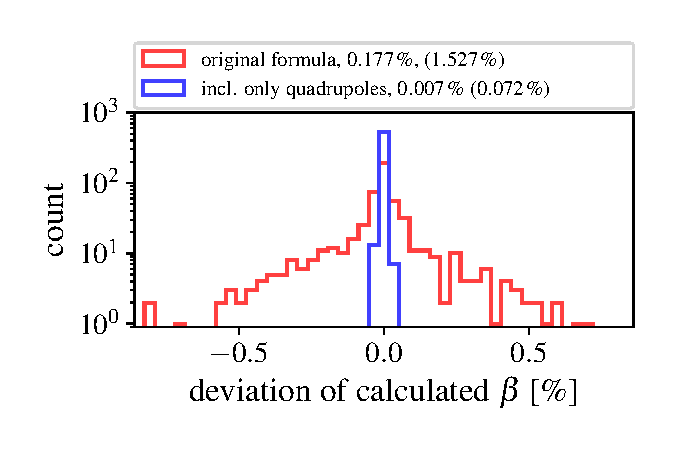
\includegraphics[width=.49\linewidth]{hist1518_ONLYQUADS_01}
  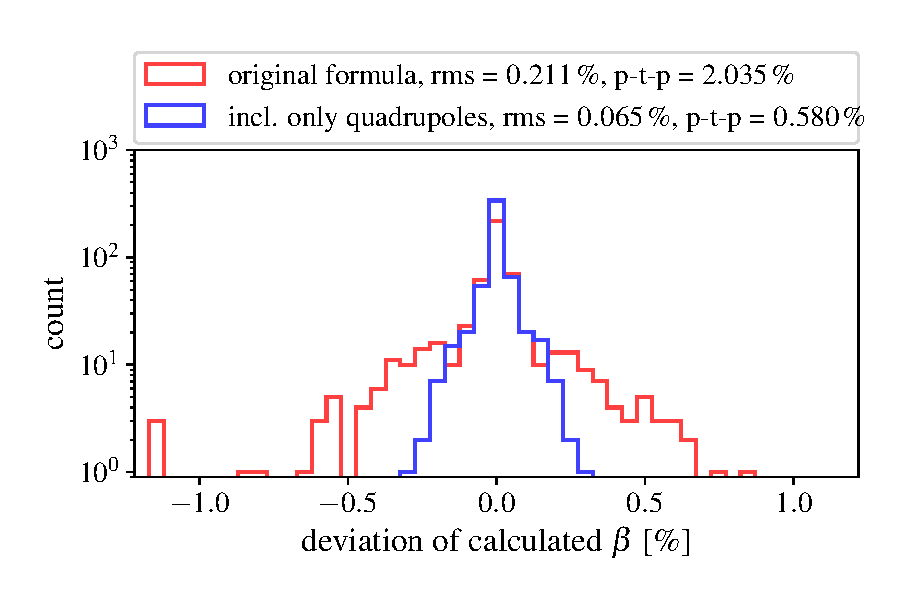
\includegraphics[width=.49\linewidth]{hist1518_NAIV_01}
	\caption{
        Left: Difference between the real (simulated) horizontal $\beta$-functions and the ones
        calculated by \eqref{eq_3bpm_method} in red and~(\ref{eq:18}) in blue, respectively. Data are from MADX
        simulations of a lattice with quadrupolar errors only.
        Right: The same quantities are evaluated for the case with additional magnet misalignments.
        the numbers which figure after the legend label show the root mean square of the deviation
        and the the peak-to-peak derivation in parenthesis.
    }
	\label{fig:hist1518}
\end{figure}
%
While the magnet misalignment errors can be approximated as \emph{effective} quadrupolar field errors
and integrated in \eqref{eq:h_ij} the BPM misalignments need a different approach as shown in the
next paragraph.

\subsection{Effect of transverse sextupole misalignments}

The magnetic field of a sextupole displaced horizontally by $ \Delta x $ reads
%
\begin{equation}
B_y = \frac{B}{2}((x + \Delta x)^2 - y^2)\quad .
\end{equation}
%
{This induces a quadrupolar field error whose strength $ \delta K_1 $ is}
%
\begin{equation}
\delta K_1 =  \left.\frac{1}{B_0\rho_0}\frac{\partial B_y}{\partial x}\right|_{x=y=0}
  = \frac{B}{B_0\rho_0}\Delta x \quad .
\end{equation}
%
This {term} can be used in \eqref{eq:h_ij} to include sextupole offsets in $ \bar{h}_{ij} $.

\subsection{Effect of longitudinal quadrupole misalignments}

%\begin{wrapfigure}{O}[\figborderhang]{8cm}
\begin{figure}
    \centering
    \includestandalone{quad_misal}
	\caption{
        The top sketch shows the displaced quadrupole (solid gray) relative to the original position
        (dashed). In the bottom sketch one can see the quadrupole at its original position with thin
        magnets on both ends.
    }
	\label{fig:quadmisal}
\end{figure}
%
The effect of a longitudinal displacement $ \delta s $ of a quadrupole magnet can be approximated by
leaving the magnet at its original position and introducing two thin magnets at its edges to mimic
the displacement, as shown in Figure~\ref{fig:quadmisal}.
The top part of the figure shows the actual situation:
The quadrupole is moved to the left such that it covers now the hatched area in addition to the gray
region. 
The bottom part illustrates the approximation method:
In the direction of the displacement there is an additional element with integrated field strength
$ \delta K_1 = k_1\delta s $ ($k_1$ being the 
non-integrated quadrupole strength), to simulate the part of the quadrupole that moved into this area
whereas an error 
$ -\delta K_1 $ is placed at the opposite end to compensate the part of the quadrupole that moved out
of this area.



\subsection{Effect of BPM misalignments}

An error, $ \delta s_i $, in the longitudinal position of
a BPM affects the evaluation of \eqref{eq:18} and \eqref{eq:h_ij} which rely on the model
values of $ \beta $ and $ \phi $ at the nominal position of the BPM.
Using \eqref{eq_phase} the phase error and the resulting $\beta$ shift at the position $s_i + \delta s_i$ can be approximated as
%
\begin{align}
\tilde{\phi}_i &\approx \phi_i + \frac{1}{\beta_i}\delta s_i\quad , 
\label{eq:Dphi} \\
\tilde{\beta}_i &\approx \beta_i + \frac{\partial \beta_i}{\partial s} \delta s_i  = \beta_i - 2\alpha_i \delta s_i \quad , \label{eq:Dbeta}
\end{align}
%
up to first order in $ \delta s_i $.

\subsection{Derivation of a corrected \texorpdfstring{$\beta$}{beta} from phase formula}

An equation similar to Eq.~(\ref{eq:18}) has to be re-derived by taking into account the considerations
of the preceding sections.

First, focusing errors, \eqref{eq_phasebeating_1st_app},
and BPM misalignments, \eqref{eq:Dphi}, are incorporated in the phase advance $\varphi_{ij}$:
%
\begin{align}
    \varphi^\text{err}_{ij}  &=
    \varphi_{ij}\m + \bar{h}_{ij} - 8\sin^2\varphi_{ij}\m\re{f_i} - 8 \sin\varphi_{ij}\m\cos\varphi_{ij}\m\im{f_i}
    + \frac{1}{\beta_j\m}\delta s_j - \frac{1}{\beta_i\m}\delta s_i \notag \\
    &= \varphi_{ij}\m + \Delta\varphi_{ij}
    \fstop
    \label{eq_phi_err}
\end{align}
%
Together with the $\beta$~shift of \eqref{eq:Dbeta}, the $\beta$~beating \eqref{eq_betabeat} and the
$\alpha$~beating,
the quotient of the first row elements of the transfer matrix, \eqref{eq_trmat_quot}, reads
%
\begin{equation}
    \frac{
        \left(m_{ij}\right)_{11}
    }{
        \left(m_{ij}\right)_{12}
    }
    =
    \frac{1}{
        (\beta_i\m - 2\alpha_i\m\delta s_i)(1-8\im{f_i})} 
    \left(
        \cot \varphi_{ij}^\text{err} +  \alpha_i(1-8\im{f_i} -8\re{f_i}) \m
    \right)
    \fstop
    \label{eq_trmat_quot_gij}
\end{equation}
%
The cotangent above can be expanded in a Taylor series around $\varphi_{ij}\m$:
%
\begin{equation}
        \cot\varphi_{ij}^\text{err}
        =\cot\varphi_{ij}\m \left( 1 - 8\im{f_i}\right) + \frac{\bar{h}_{ij}}{\sin^2\varphi_{ij}\m} - 8 \re{f_i}
        + \frac{\frac{1}{\beta_i\m}\delta s_i + \frac{1}{\beta_j\m}\delta s_j}{\sin^2\varphi_{ij}\m}
\end{equation}
%
and \eqref{eq_trmat_quot_gij} can be simplified:
%
\begin{align}
    \frac{
        \left(m_{ij}\right)_{11}
    }{
        \left(m_{ij}\right)_{12}
    }
    =
    \frac{1}{\beta_i\m - 2\alpha_i\m\delta s_i} 
    \left(
        \cot \varphi_{ij}^\text{err} + \alpha_i \m + \bar{g}_{ij}
    \right)
\end{align}
%
with 
%
\begin{equation}
\bar{g}_{ij} = \text{sgn}(i-j)\dfrac{ \frac{1}{\beta\m(s_j)}\delta s_j - \frac{1}{\beta\m(s_i)}\delta s_i +
\sumw\beta_w\m\delta K_{w,1}\sin^2\phi_{wj}\m}{\sin^2\phi_{ij}\m}\quad ,
\label{eq:g_ij}
\end{equation}
%
To get the corrected $\beta$ from phase formula one has to follow the same steps as in section~\ref{sec_beta_meas}:
%
\begin{align}
    \frac{\left(m_{ij}\right)_{11}}{\left(m_{ij}\right)_{12}} - \frac{\left(m_{ik}\right)_{11}}{\left(m_{ik}\right)_{12}}
    =&
    \frac{1}{\beta_i} \left( \cot\varphi_{ij} - \cot\varphi_{ik}\right)
    %\notag \\
    -
    \frac{1}{\left(\beta_i\m - 2\alpha_i\m \right) } 
    \notag \\
    &\times\left[
        \cot\varphi_{ij}\m  + \bar{g}_{ij}
        -
        \cot\varphi_{ik}\m  - \bar{g}_{ik}
    \right]
\end{align}
%
and the final expression for the $\beta$~function at position $s_i$ from the combination $l$ reads
%
\begin{align}
\beta_l(s_i) \approx& \frac{\cot\phi_{i{j_l}} - \cot\phi_{i{k_l}}}{\cot\phi_{i{j_l}}\m - \cot\phi_{i{k_l}}\m +\bar{g}_{i{j_l}} - \bar{g}_{i{k_l}}} \left[\beta\m(s_i) - 2 \alpha\m(s_i) \delta s_i\right]
    \fstop
\label{eq:beta_g}
\end{align}
%
In order to account for sextupole misalignments and quadrupole longitudinal misalignments, it suffices
to add the corresponding effective $\delta K_1$ to the sum in $\bar{g}_{ij}$,
as described in the previous sections. 
The set $I$ is defined in~\eqref{eq_def_sgn_fun},
so that an element with index $ w \in I$ lies between elements $ i $ and $ j $
and Eqs~(\ref{eq:beta_g}) and~(\ref{eq:g_ij}) hold for every BPM combination $ i $, $ j $, $ k $.
%
\begin{figure}
	\centering
  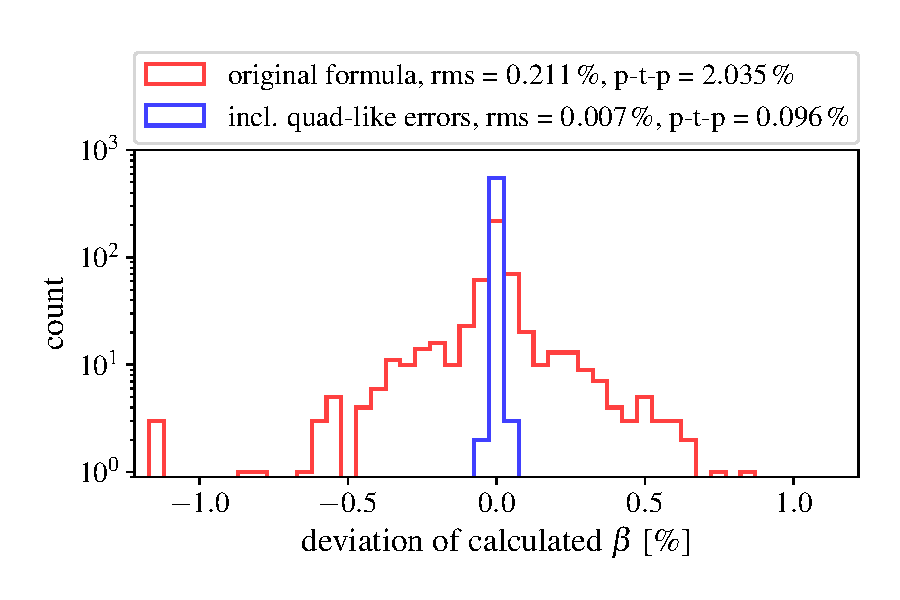
\includegraphics[width=.7\linewidth]{hist1518_EVERYTHING_01}
    \caption{Accuracy of the horizontal $\beta$-function evaluated via \eqref{eq_3bpm_method} and~\eqref{eq:beta_g} with the effect of magnets and BPM misalignments taken into account. The accuracy of
 \eqref{eq:beta_g} is similar to the one of \eqref{eq:18} with quadrupolar field errors only (Figure~\ref{fig:hist1518}).}
	\label{fig:hist1518_with_everything}
%\end{wrapfigure}
\end{figure}
%
By doing so, we do not need to distinguish the three cases where the probed BPM is in the middle, left or right.

All these considerations can be put into \eqref{eq:beta_g} and used to get a more accurate
$ \beta $ function.
To verify the validity of \eqref{eq:beta_g}, its horizontal $\beta$-functions are compared to the
ones simulated by MADX along with the ones inferred from \eqref{eq_3bpm_method}, this time including
sextupole radial offsets and BPMs longitudinal shifts.

The result is shown in Figure~\ref{fig:hist1518_with_everything}. The accuracy is now as good as the one of \eqref{eq:18}  when only quadrupolar field errors were introduced in the
lattice, which in turn is much greater than the old formula, \eqref{eq_3bpm_method}.

\section{Calculation of the correlation matrix}
\label{sec_corr_matr}

The Jacobian $ \mathbf{T} $ of \eqref{eq:Tij} can be split into blocks 
%
\begin{equation}
\mathbf{T} = \left( \mathbf{T}^\phi \quad \mathbf{T}^K \quad \mathbf{T}^s\right),
\end{equation}
%
for the uncertainties of phase $ \mathbf{T}^\phi$, quadrupole field  $\mathbf{T}^K$ and BPM misalignment $\mathbf{T}^s$.
$ \mathbf{T}^\phi $ is the same of \eqref{eq:Tphiij}. For the quadrupolar field errors we get
%
\begin{align}
	T^K_{l\lambda}(s_i) = 
		\left. \frac{\partial \beta_l(s_i)}{\partial  K_{1,\lambda}}\right|_{\delta K = 0} =
		\mp\frac{\beta\m(s_i)\beta\m(s_\lambda)}{\cot\phi_{ij_l}\m - \cot\phi_{ik_l}\m}\left(
		\frac{\sin^2\phi_{\lambda j_l}\m}{\sin^2\phi_{ij_l}\m}A_{ij_l}(\lambda) - \frac{\sin^2\phi_{\lambda k_l}\m}{\sin^2\phi_{ik_l}\m}A_{jk_l}(\lambda)\right)\quad ,
\label{eq:TK}
\end{align}
%
  with 
%
\begin{equation}
    A_{ij}(\lambda) = \left\{\begin{array}{ll}
    1&\text{if }i<\lambda<j\\
    -1&\text{if }j<\lambda<i\\
    0&\text{else}
    \end{array}\right. \quad .
  \end{equation}
%
  The contribution from the BPM misalignment is calculated analogously:
%
\begin{align}
      T^s_{l\lambda}(s_i) &= \left.\frac{\partial \beta_l(s_i)}{\partial s_\lambda}\right|_{\delta s = 0} \notag \\
      &= -2\alpha^m(s_i)\delta_i^{\lambda}
      \mp 
      \frac{
          \dfrac{\text{sgn}(i-j_l)}{\sin^2 \phi_{ij_l}\m}\left(\dfrac{\beta\m(s_i)}{\beta\m(s_{j_l})}\delta^{j_l}_\lambda - \delta_\lambda^i\right) -
          \dfrac{\text{sgn}(i-k_l)}{\sin^2 \phi_{ik_l}\m}\left(\dfrac{\beta\m(s_i)}{\beta\m(s_{k_l})}\delta^{k_l}_\lambda - \delta_\lambda^i\right)}
      {\cot \phi_{ij_l}\m - \cot \phi_{ik_l}\m} \quad .
      \label{Ts}
  \end{align}
%
  In \eqref{eq:TK} and~\eqref{Ts} the minus and plus signs refer to the horizontal and vertical case, respectively. 
%In Equations~(\ref{eq:TK}) and~(\ref{Ts}) $\delta \epsilon = 0$ means \[\delta K_w = \delta s_w = \delta \phi_w = 0,\quad \forall w.\]

\section{Removal of bad BPM combinations}
\label{sec_bad_combs}


\begin{figure}
	\centering
    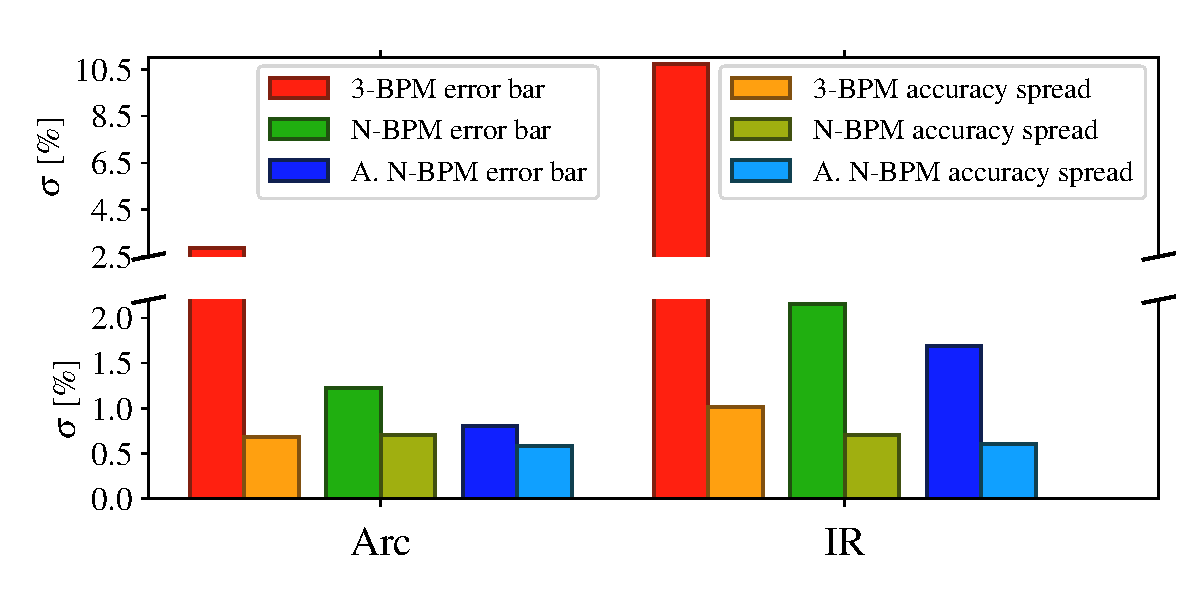
\includegraphics[width=.7\linewidth]{comparison_statistics_007_bars}
    \\
    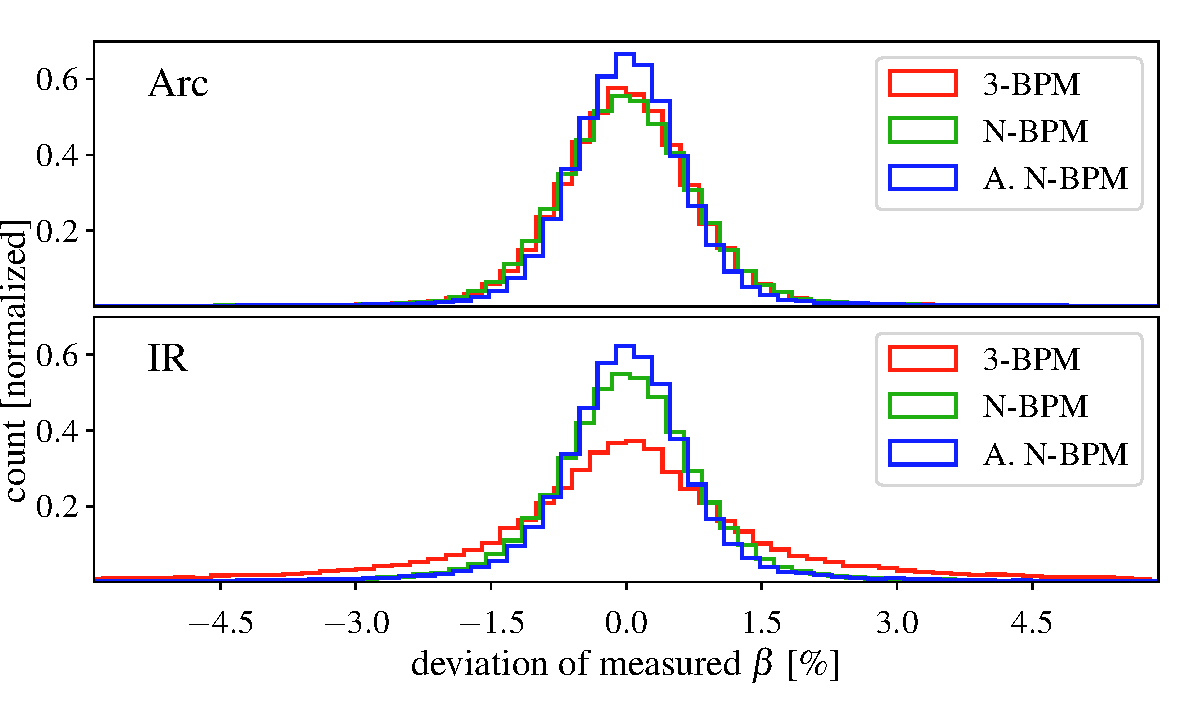
\includegraphics[width=.7\linewidth]{comparison_statistics_006}
	\caption{Comparison of the 3-BPM method, the original N-BPM method and the analytical N-BPM method (denoted as \texttt{A.N-BPM}) for the nominal LHC lattice at collision, with $ \beta^*=40\,\text{cm} $. BOTTOM: histogram of the difference to the real $\beta$-function in percent. TOP: the average of the error bars and the accuracy spread (width of a standard distribution fit to the distribution in the bottom plot) in percent.  The analytical N-BPM method has the best accuracy both in the arcs and in the IRs. Data have been cleaned of outliers.}
	\label{fig:compare_NBPM_to_3BPM}
\end{figure}
%
\begin{figure}
	\centering
    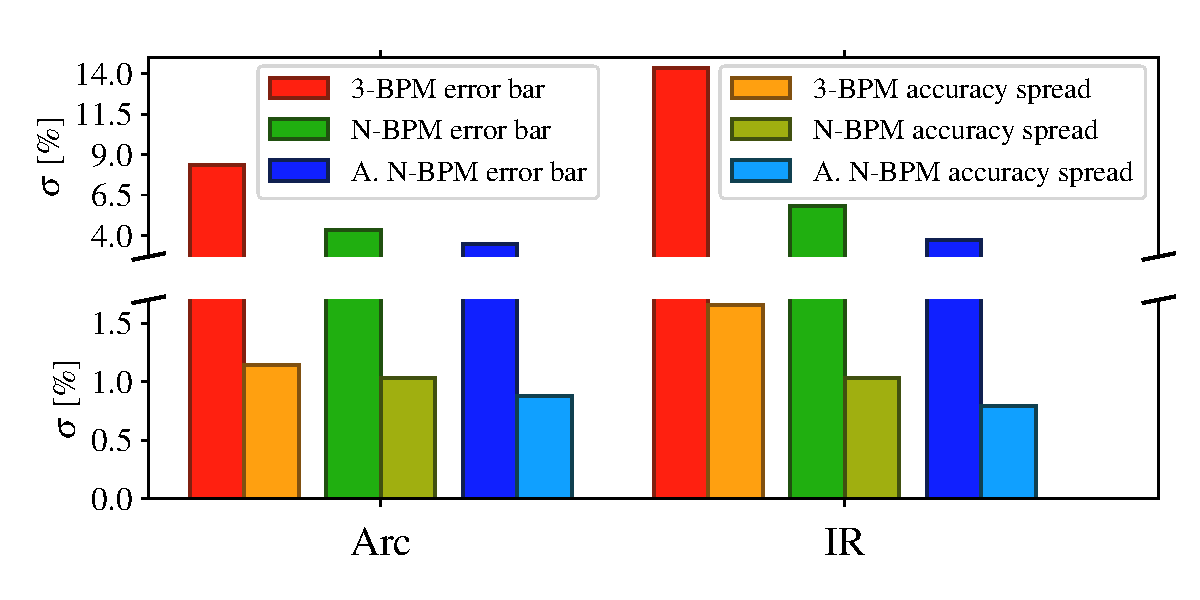
\includegraphics[width=.7\linewidth]{comparison_statistics_HL007_bars}
    \\
    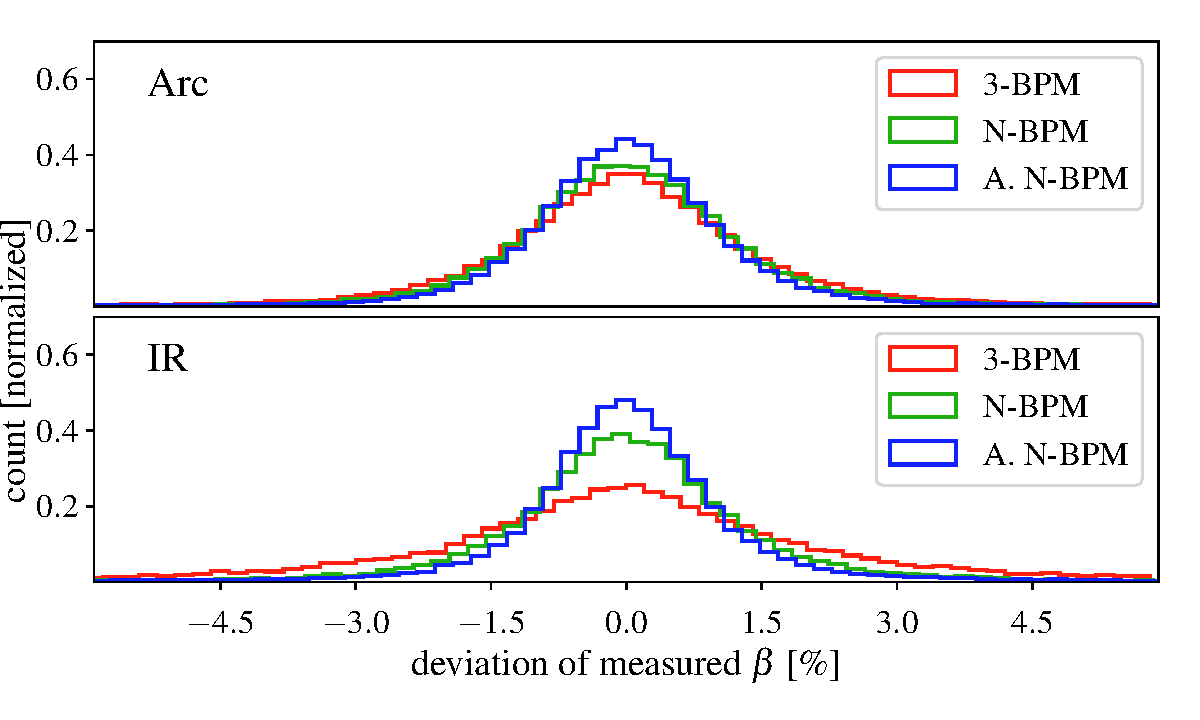
\includegraphics[width=.7\linewidth]{comparison_statistics_HL006}
	
	\caption{
        Same comparison of Figure~\ref{fig:compare_NBPM_to_3BPM} between the three methods for the
        HL-LHC $ \beta^*= 15\,\text{cm} $ ATS optics. The analytical N-BPM method yields clearly
        better results, both in the IRs and in the arcs. Compared to the $ \beta^*=40\,\text{cm} $
        optics shown in Figure~\ref{fig:compare_NBPM_to_3BPM}, the $ \beta $ function reconstruction
        is less accurate: This was also demonstrated for the $ \beta^*=20\,\text{cm} $ optics in
        \cite{LangnerNBPM}. }
	\label{fig:compare_ATS}
\end{figure}
%
\begin{figure}
	\centering
    %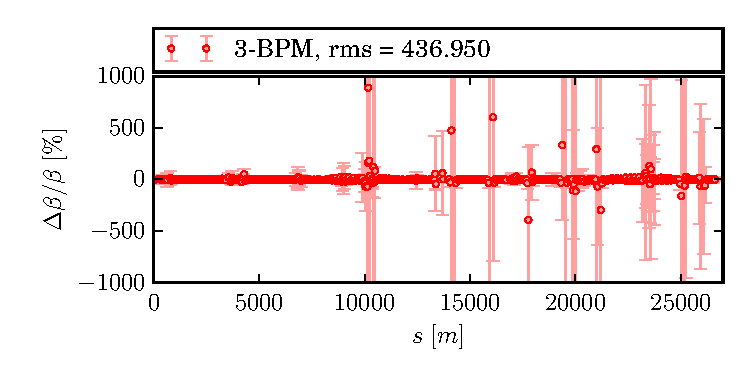
\includegraphics[width=.7\linewidth]{10cm_b1_x_3bpm}
    %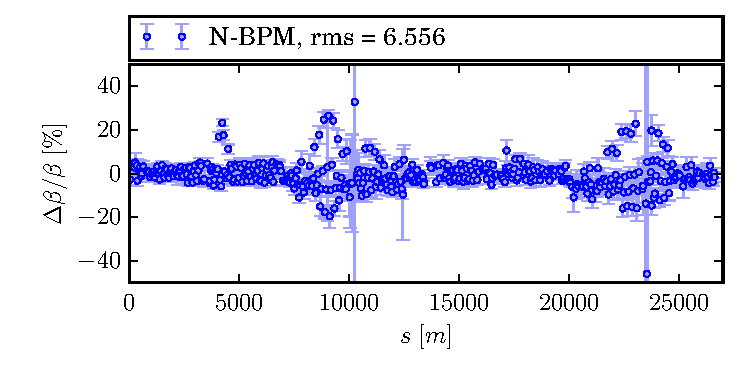
\includegraphics[width=.7\linewidth]{10cm_b1_x_nbpm}
    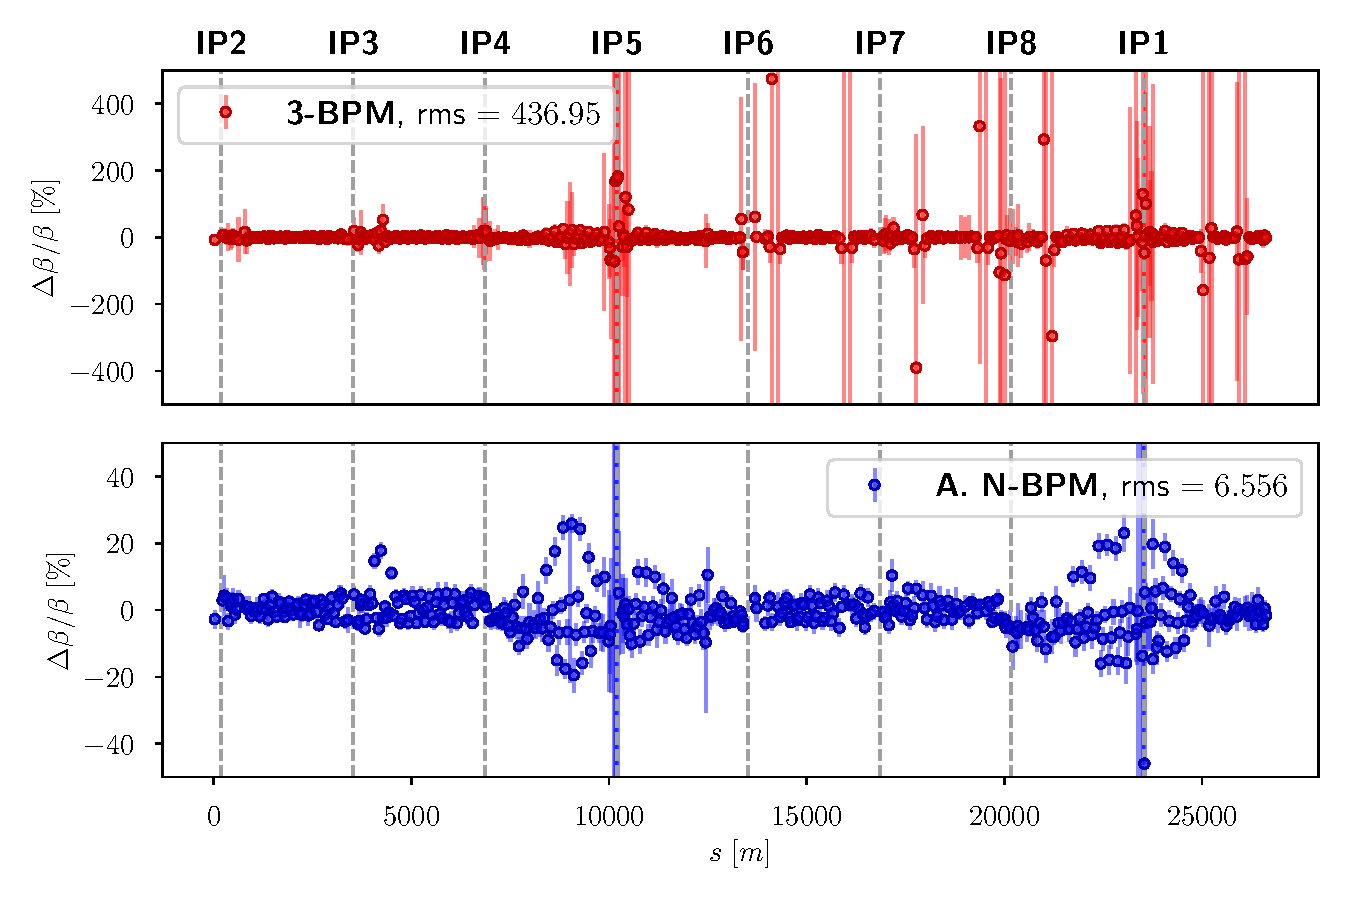
\includegraphics[width=0.9\linewidth]{2021_ATS10cm_001}
	\caption{Horizontal $ \beta $ beating of beam 1 at $ \beta^*=10\,\text{cm} $ during the ATS MD 2016. TOP: 3-BPM method. BOTTOM: analytical N-BPM method. The 3-BPM method suffers from bad phase advances and has many outliers. The regions of high $ \beta $ beating at around $ \SI{8000}{m} $ and $ \SI{23000}{m} $ lie in the telescopic arcs. }
	\label{fig:10cm_beam1_hor_3bpm}
\end{figure}
%
\begin{figure}
	\centering
	%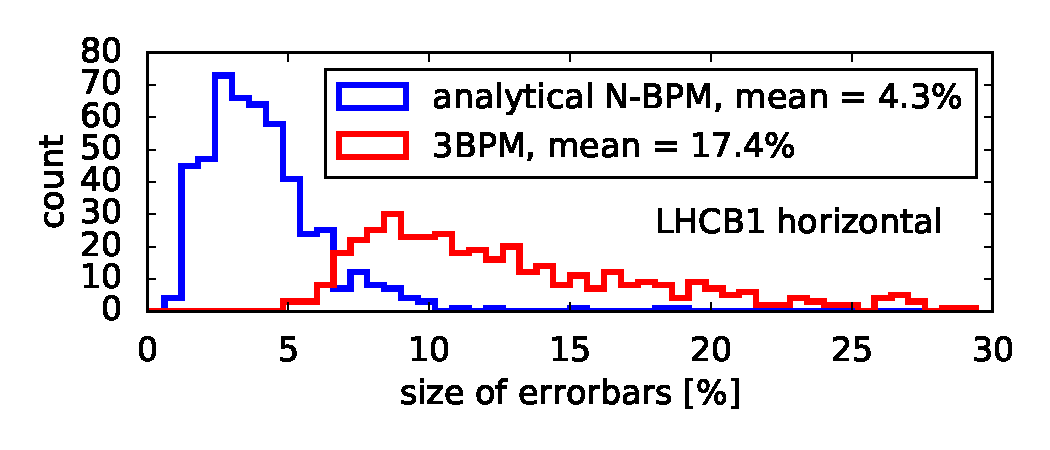
\includegraphics[width=.49\linewidth]{comparison_errorbars_Beam1}
	%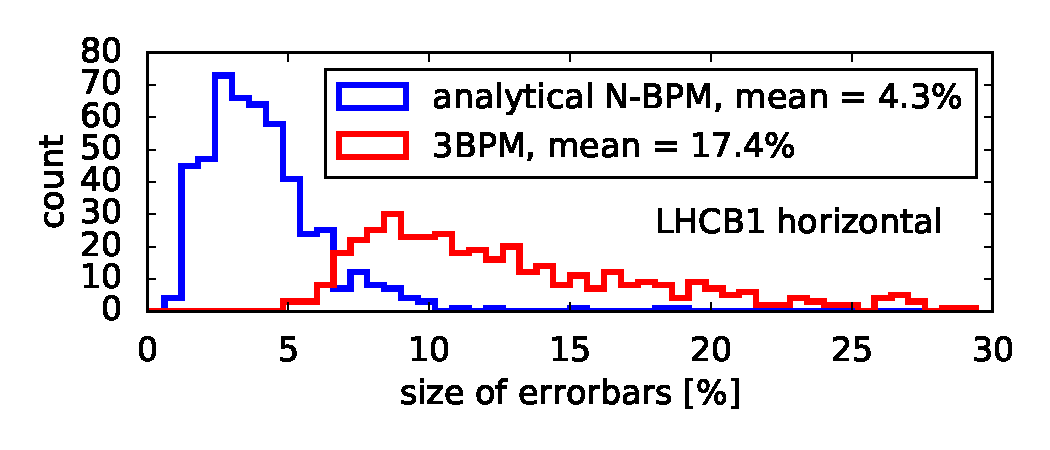
\includegraphics[width=.49\linewidth]{comparison_errorbars_Beam2}
    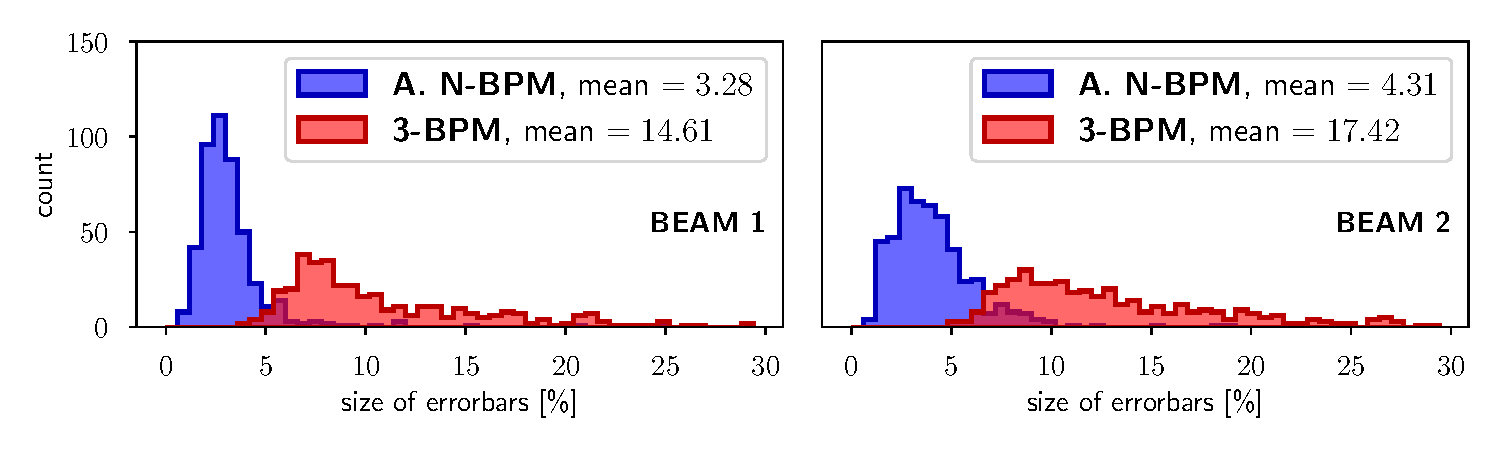
\includegraphics[width=0.9\linewidth]{2021_ATS10cm_histo}
	
	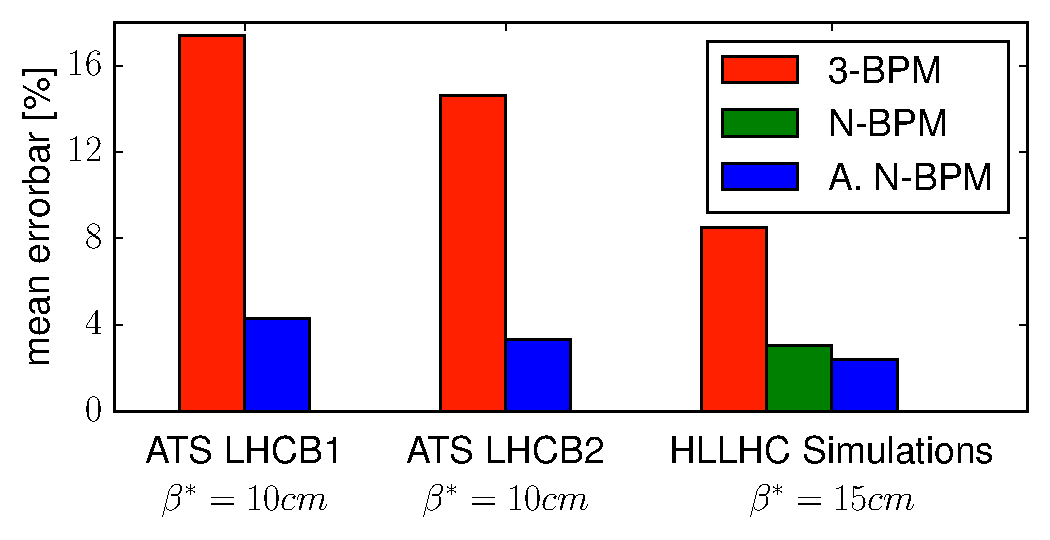
\includegraphics[width=.6\linewidth]{mean_errorbars}
	
	\caption{
        A comparison of the error bars of the $ \beta^*=10\,\text{cm} $ optics of the October 2016 MD.
        TOP LEFT: histogram of the error bars of beam 1. TOP RIGHT: histogram of the error bars of beam 2.
        BOTTOM: mean of the size the error bars. The mean of the analytical N-BPM method is a factor
        4 more accurate than the 3 BPM method. The third set of values shows the mean of the error bars
        of the simulations as shown in Figure~\ref{fig:compare_ATS} but for the whole ring.
        }
	\label{fig:HL_report/comparison_errorbars}
\end{figure}
%
Since a phase advance $ \phi_{ij} \approx n\pi $ results in an enhancement of phase measurement errors and in the extreme case numerically unstable values, a filtering was introduced. Instead of keeping a constant number of combinations as in \cite{LangnerNBPM} we set a threshold for \emph{bad} phase advances. A phase advance $ \Delta \phi $ is considered \emph{bad} if $ \Delta \phi \in [ n\pi - \delta, n\pi + \delta ] $ for $ n\in \mathbb{N} $ and a given threshold $ \delta $. If any of the four phase advances $ \phi_{ij_l}, \phi_{ik_l},\phi_{ij_l}\m,\phi_{ik_l}\m $ in Eq.~\eqref{eq_3bpm_method} is bad, the corresponding BPM combination is disregarded in the calculation of the weighted mean. This allows us to still use several combinations but skipping those which are numerically unstable. The current value for the threshold is $ \delta = 2\pi \cdot 10^{-2}$. The use of fewer combinations results in a lower computation time. 


To test the analytical N-BPM method and compare it to the original 3-BPM and the Monte Carlo N-BPM
method, a large set of LHC lattices with $ \beta^*=40\,\text{cm} $ with randomly distributed errors
is generated and a measurement is simulated by tracking a single particle via polymorphic tracking
code (PTC) \cite{Schmidt2002}. The random errors are created from table \ref{tab:unc_estimates}
and a Gaussian noise of $ \sigma_x = 0.1\,\text{mm} $ is applied to the BPM signal. No singular value
decomposition cleaning is applied since it would clean the artificial noise too efficiently
\cite{Langner2016}. The excitation amplitude is $\SI{0.8}{mm}$ at a $ \beta $ function of about
$ \SI{120}{m} $. The tracked particle positions are then analyzed by the three methods
(3-BPM, N-BPM and analytical N-BPM) and the respective deviation from the real horizontal
$ \beta $ function is shown in the bottom plot of Figure~\ref{fig:compare_NBPM_to_3BPM}.
The analytial N-BPM method includes the filtering of phase advances. Especially in the IR, where
neighbouring BPMs have often unsuitable phase advances, the N-BPM and analytical N-BPM method yield
more accurate values.

The top diagram of Figure~\ref{fig:compare_NBPM_to_3BPM} shows that the error of the 3-BPM method is considerable larger, whereas the N-BPM and analytical N-BPM method are very accurate with similar accuracies in the IR and arcs.


\section{HL-LHC}
\label{sec_hllhc_nbpm}
The ATS optics \cite{Fartoukh2013} is the baseline choice for the HL-LHC and our optics measurement
tools have to be prepared for the challenges imposed by such an optics. In Figure~\ref{fig:compare_ATS}
the three methods are compared in the same way as in Figure~\ref{fig:compare_NBPM_to_3BPM}.
The excitation amplitude was $ \SI{0.8}{mm} $ at a $ \beta $ function of $ \SI{127}{m} $.
For the current HL-LHC collision optics ($ \beta^* =15\,\text{cm}$) the performance of N-BPM and
analytical N-BPM method is again better than the 3-BPM method, especially in the IRs. All three
methods are, however, about a factor two more inaccurate than for the $ \beta^*=\SI{40}{cm} $ optics
of LHC, in agreement with Figure~7 of \cite{LangnerNBPM}.

In the post-processing of the data taken during the LHC Machine Development
measurement (MD) \cite{mdpubl} for testing the ATS principle with a $ \beta^* = 10$ cm optics, the analytical N-BPM method was used for the first time with filtering of bad phase advances. Figure 7 demonstrates that the analytical N-BPM
method deals well with the ATS MD optics. Monte Carlo simulations were
not possible for this optics.

Figure~\ref{fig:HL_report/comparison_errorbars} shows the precision of the final results for the $ \beta^*=10\,\text{cm} $
optics of both beams compared to the simulations of the HL-LHC lattice with $ \beta^*=\SI{15}{cm} $.
To ease the comparison the error bars are shown in the bottom plot.
They are slightly larger for the real measurement than those in simulations.
We believe that the use of lower beam excitation to ensure machine protection is behind these larger error bars.
Figure~\ref{fig:10cm_beam1_hor_3bpm} shows also that the 3-BPM method has many outliers and error bars up to several
kilometers caused by bad phase advances. Large error bars have been excluded for the mean shown in
Fig.~\ref{fig:HL_report/comparison_errorbars}.



The Monte Carlo simulations failed for low $ \beta^* $ optics and so we were not able to use the original N-BPM method during ATS MDs. This is another advantage of the analytical N-BPM method that it is
able to evaluate the systematic errors independently of the success of particle tracking.

\section{Conclusion}
\label{sec_nbpm_concl}

A new method for the measurement of $\beta$ and $\alpha$~functions has been
developed based on the existing N-BPM method.
A fully analytical calculation of the covariance matrix provides a faster and more accurate measurement
of $ \beta  $ and $ \alpha $ functions. The analytical N-BPM method also avoids the complications from
failing to find closed optics that occur in the Monte Carlo simulations  needed by the existing N-BPM method.
This stability with respect to the choice of optics model makes it more suitable for low $ \beta^* $~optics.
Simulations show that, together with a filtering of BPM combinations according to the phase advances,
the method is optimal for the HL-LHC upgrade. 

In the last years, the analytical N-BPM method has been used as standard method to measure the $\beta$~function in LHC
beam commissionning and machine development studies where it has been producing a high quality analysis
and contributed to the remarkable performance of the LHC in run~II.
The method also has been used in collaborative efforts
with accelerators from several external institutes like SuperKEKB (KEK) and PETRA~III (DESY). 
